
\section{Hardware Implementation}
\label{sec:implementation}

Although a completed and detailed floorplan of the node is not the
focus of this work, in this section we want to give a basic idea of
which are the main elements required to support this kind of
architecture thus giving an estimate of the overhead by the
DiSR approach. There are three main classes of node elements:
\begin{itemize}
\item Node-specific: components (such ALUs, memories) that are
strictly related to the node functionality and role inside a given
network, e.g. being a computation or storage node.
\item Node communication:  these are elements (such as transceivers,
buffers) required to the node to communicate with its neighbours,
independently from node functionality and DiSR implementatio
\item DiSR-specific: all the hardware, control logic and
configuration registers, related to an implementation the proposed approach.
\end{itemize}

\begin{figure}
  \centering
  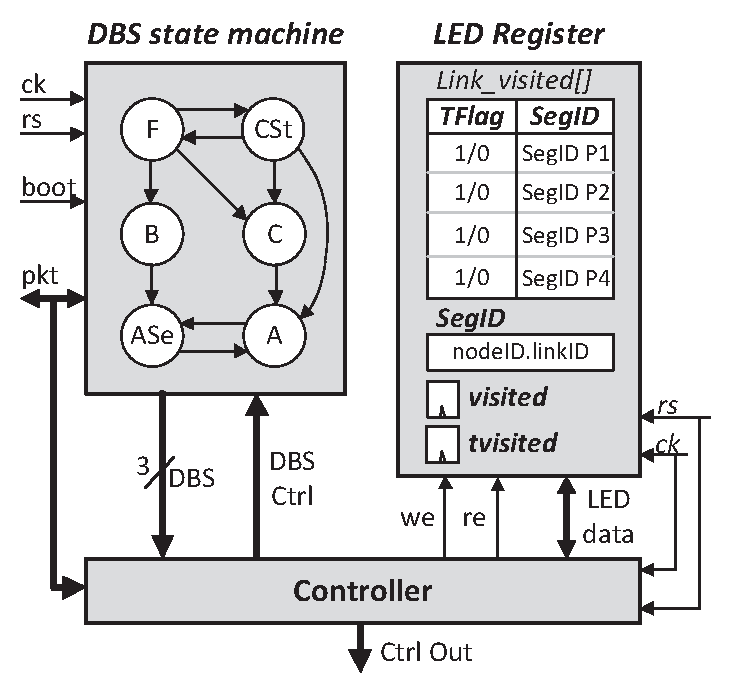
\includegraphics[width=0.40\textwidth]{pictures/implementation.eps}
  \caption{\emph{DiSR} block architecture.}
 \label{fig:implementation}
\end{figure}

To give a basic estimate of the overhead needed we will focus on
DiSR-specific components, that is, the control logic and configuration
registers needed to implement DiSR. In
Figure~\ref{fig:implementation} is shown a sketch of this block, which
mainly consist in the following building element: 
\begin{itemize}
	\item \textbf{DBS block:} It takes trace of the DBS state machine, 
	consisting of a 3-bit register (to cover six DBS values) and the 
	required combinational logic. This block receives signals from 
	stored packets to decode the packet type, and from 
	the control circuitry to change its status.
	The bootstrap node is selected by setting the boot signal to high
	during the initialization phase.  
	\item \textbf{LED registers:} A set of registers storing 
	the Local Environment Data (LED) listed in the section
	\ref{sec:disr_concepts}. It should be pointed out that, while the \emph{visited} 
	and \emph{tvisited} data must be implemented with two distinct
	elements, the \emph{tvisited} and \emph{visited} table can be implemented with 
	a single RAM file for storing the segment id of each link.
	This can be done adding a special register named \emph{Tflag}
	indicating whether the \emph{SegID} value refers to \emph{visited} or to 
	\emph{tvisited}. When SegID's register is set to 0, it means that the link
	is neither visited nor tvisited.

    \item \textbf{Control circuitry:} This circuitry reads data from
	the incoming packet, the LED registers and the DBS,
	updating them when required. This block drives the LED register 
	for storing or, for reading the LED data according with
	\emph{write enable (WE)} or \emph{read enable (RE)}
	signals. Then, the resulting Ctrl-Out output drives the other
	communication resources for actuating the DiSR routing operation.
\end{itemize}

Each building block reacts with the rising edge  of
the\emph{clock signal} shown in Figure. An asynchronous system
\emph{reset} signal is also present for restoring all registers to
their default values. When this last signal is
set, the DBS state machines for each network's node are set as
\emph{Free}. 

As discussed above, one of the main design challenge of DNA
Self-Assembled systems is the limited resource available for
implementing both computations and routing decisions for each node.
Assuming a budget of $10^4$ CNFETs for each network's
node~\cite{liu_jetcs}  we estimated the required resource for
implementing the entire DiSR block.  A not optimized RTL description
(with an hardware description language)  of the DiSR circuitry has
been written and synthesized at gate-level. Considering the specific
layout of each single logic elements (NAND, full-adder, latch etc.),
it has been possible to get a rough estimate of the number of
transistors necessary for implementing the DiSR logic.

Figure~\ref{fig:imp_trend} shows the results of synthesis in
terms of number of devices (CNFETs) versus the number of network nodes
while the network scales up from $10\times10$ to $100\times100$ nodes.
\begin{figure}
  \centering
  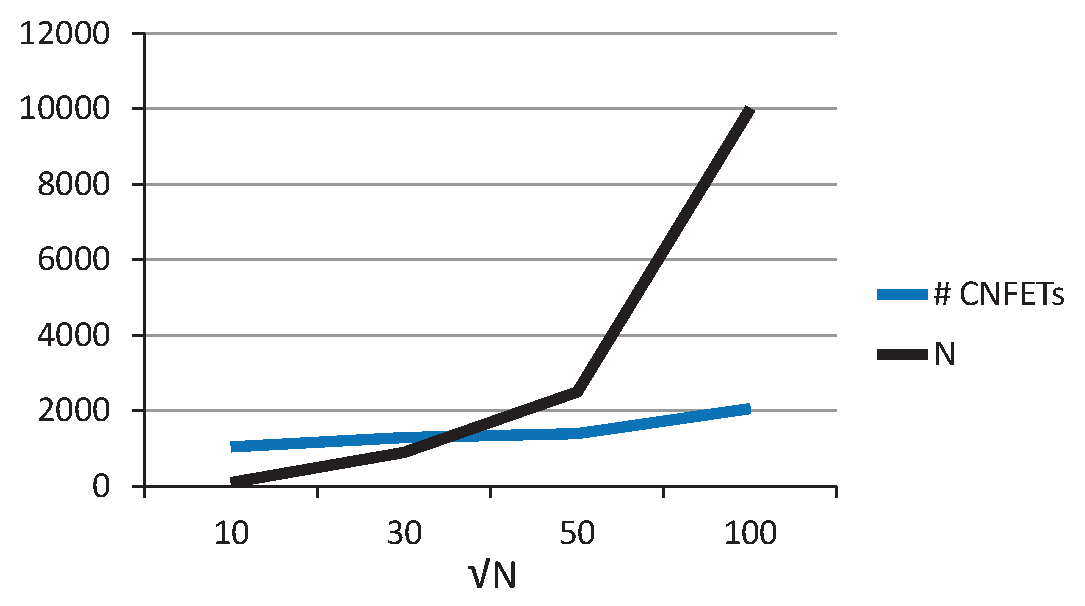
\includegraphics[width=0.40\textwidth]{pictures/imp_rslt.eps}
  \caption{Number of network's node (N) vs number of CNFETs.}
 \label{fig:imp_trend}
\end{figure}
In particular, observing the Figure~\ref{fig:imp_trend} can 
be pointed out that the proposed implementation occupy  about 17\% of the node budget. 
Further, more than the absolute number of devices itself, it is interesting to
observe that, while the node have a squared increment, the circuitry
complexity which implements the DiSR algorithm increases with a slowly
growing trend.  
An intuitive explanation of this is the relatively simple logic of
DiSR, whose behaviour is al4ost code on scalable storage structures.
For example, the number of registers
implementing the \emph{link\_visited[]} and \emph{link\_tvisited[]}
table follow the logarithmic function $N_{reg}=N_{port} \cdot
log_2(N)$ where \emph{Nport} is the number of the router’s ports, N is
the number of network’s nodes.  While $N_{reg}$ is fixed by the number
of network’s node,  the control circuitry could be optimized applying
more effort in future designs of this building block.

